\chapter{Porting of a wide band waveform}

\section{IEEE 802.11g}

\subsection{Overview of Wireless LAN}
Since 1980, the \ac{IEEE} releases specification about Local Area Networks (LANs) in its project 802. In 1997, the first specification of an \ac{WLAN} was published within the working group eleven. Hence the standard IEEE 802.11 was created, that specifies \ac{MAC} and \ac{PHY} for local radio networks. In this original version, data rates up to 2 Mbit/s were reached with spread spectrum techniques in the 2.4 GHz \ac{ISM} radio band. Just about two years later, in 1999, the standard was extended with two annexes. IEEE 802.11a specified an \ac{OFDM} transmission in the 5 GHz \ac{ISM} band with data rates up to 54 Mbit/s and 802.11b extended the transmission on 2.4 GHz to data rates up to 11 Mbit/s. The most common extension till the present day is annex g, that was released in 2003 and specified the \ac{OFDM} transmission with up to 54 MBit/s in the 2.4 GHz range.

\subsection{Frame Structure}
The interoperability and compatibility between the different extensions of the 802.11 family is given through its remaining frame structure. In a wireless connection according to the \ac{WLAN} specification, transmitter and receiver exchange \texttt{\acp{PPDU}}. These are frames, consisting of a defined preamble, signaling information and a field for the payload as depicted in figure \ref{fig:ppdu}. 

\begin{figure}[ht]
	\centering
		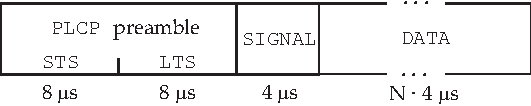
\includegraphics{../kapitel04/figures/ppdu.pdf}
	\caption{Structure of the \texttt{PPDU}}
	\label{fig:ppdu}
\end{figure}

\subsubsection{\texttt{PLCP} preamble}
The preamble of the \texttt{\ac{PLCP}} consists of two training sequences: the \texttt{\ac{STS}} and the \texttt{\ac{LTS}}. The \texttt{\ac{STS}} shall be used by the receiver to detect the \texttt{\ac{PPDU}}, tune the \ac{AGC}, and synchronize the time and frequency offset coarsely. It is  defined in the frequency range as twelve active subcarriers modulated by a sequence defined in clause 17-6 in \cite{IEEE802.11}. Note the factor of $\sqrt{\nicefrac{13}{6}}$ in order to normalize the average power of the OFDM symbol that does only utilize 12 of 52 subcarriers. The fact, that only every fourth carrier is occupied in the frequency domain leads to periodicity of \SI{0.8}{\micro s} and hence to ten periods in the time domain. The \texttt{\ac{STS}} is depicted in figure \ref{fig:STS} in frequency and time.

\begin{figure}[ht]
	\centering
		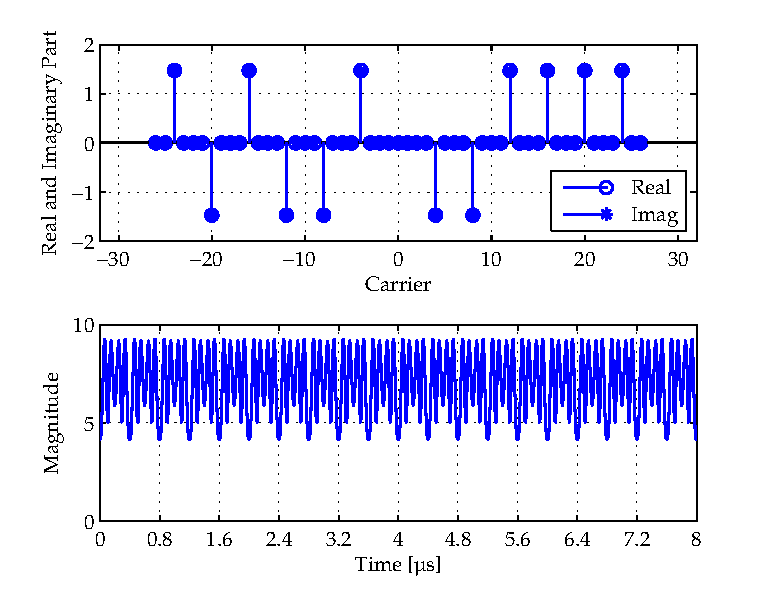
\includegraphics[width=1.00\textwidth]{../kapitel04/figures/STS.pdf}
	\caption{The \texttt{STS} in the frequency and time domain}
	\label{fig:STS}
\end{figure}

The \texttt{\ac{LTS}} is also defined in the frequency range with clause 17-8 in \cite{IEEE802.11}. Unlike the definition of the \texttt{\ac{STS}}, every subcarrier is used and hence no normalization factor is needed. The representation in the time domain can be accessed with the discrete fourier transformation and is depicted in figure \ref{fig:LTS}. The mandatory duration of  \SI{8}{\micro s} for the \texttt{\ac{LTS}} leads to two periods of \SI{3.2}{\micro s} with a guard interval of \SI{1.6}{\micro s}. This enables improved channel estimation accuracy and a fine frequency synchronization. 

\begin{figure}[ht]
	\centering
		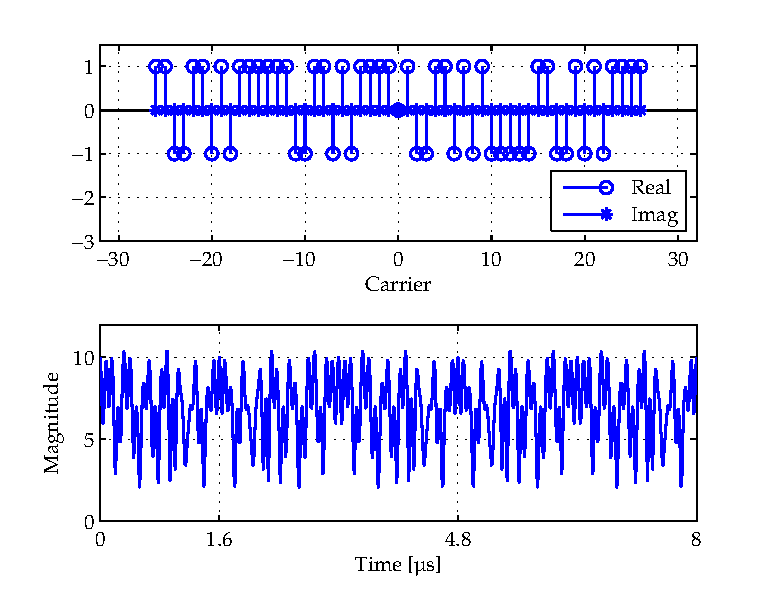
\includegraphics[width=1.00\textwidth]{../kapitel04/figures/LTS.pdf}
	\caption{The \texttt{LTS} in the frequency and time domain}
	\label{fig:LTS}
\end{figure}


\subsubsection{\texttt{SIGNAL} field}

The \texttt{SIGNAL} field provides the information about the length and data rate of the \texttt{DATA} field. Without these informations, the receiver is not able to decode and has to drop the whole \ac{PPDU}. To assure a robust transmission, the \texttt{SIGNAL} field is modulated with BPSK and encoded with a rate $\nicefrac{1}{2}$ convolution encoder. This fix modulation and coding scheme leads to 24 bits per \texttt{SIGNAL} field as depicted in figure \ref{fig:SIGNAL_Frame}. The first four bits shall encode the data rate of the \texttt{DATA} field, which consists of the combination of modulation scheme, coding scheme and puncturing. The number of payload octets is indicated by twelve bits as can be seen in figure \ref{fig:SIGNAL_Frame} in the \texttt{LENGTH} field. The 17th bit shall be a positive parity bit for the first 16 bit while the the bits 18-25 shall be set to zero.
 
\begin{figure}[ht]
	\centering
		\includegraphics{../kapitel04/figures/SIGNAL_Field.pdf}
	\caption{Structure of the \texttt{SIGNAL} Field}
	\label{fig:SIGNAL_Frame}
\end{figure}

\subsubsection{\texttt{DATA} field}

The \texttt{DATA} field contains the \texttt{SERVICE} field, the \texttt{\ac{PSDU}}as well as \texttt{TAIL} bits and if necessary \texttt{PAD} bits as depicted in figure \ref{fig:data_field}. The SERVICE field has 16 bits that shall be set to zero. The first six bits are used to synchronize the descrambler in the receiver while the following nine bits are reserved for future use. The data in the PSDU field is the payload of the actual transmission with a length of $N_{PSDU}$ bits. The relation to the LENGTH field is given by:
\begin{equation}
	N_{PSDU} = 8 \cdot \texttt{LENGTH}
\end{equation}
To assure that the convolutional encoder returns to the zero state, the TAIL field with six 0-bits has to be attached to the PSDU. The PAD field is finally used to assure that the length of a message becomes a multiple of $N_{DBPS}$, the number of data bits per \ac{OFDM} symbol. Therefore its length $N_{PAD}$ is given by:




\begin{equation}
N_{PAD} = \left\lceil \frac{16 + N_{PSDU} +6 }{N_{DBPS}} \right\rceil \cdot N_{DBPS} - \left ( 16 + N_{PSDU} + 6  \right )
\end{equation}

\begin{figure}[ht]
	\centering
		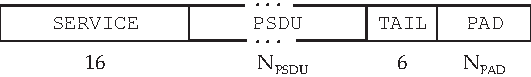
\includegraphics{../kapitel04/figures/Data_Field.pdf}
	\caption{Structure of the \texttt{DATA} field}
	\label{fig:data_field}
\end{figure}


\subsection{MAC Layer}

\begin{figure}[ht]
	\centering
		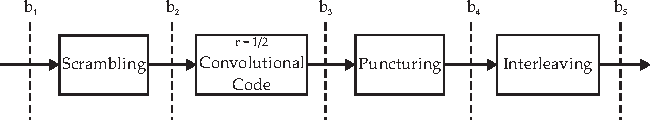
\includegraphics[width=1.00\textwidth]{../kapitel04/figures/MAC_IEEE.pdf}
	\caption{Structure of the MAC}
	\label{fig:MAC_IEEE}
\end{figure}


The bits in the \texttt{DATA} field shall be scrambled by adding a pseudo noise sequence $p$:
 
\begin{equation}
b_2(k) = b_1(k) + p(k) = b_1(k) + \sum_{i=1}^{7}c_i p(k-i)
\label{pn_ieee}
\end{equation}
The coefficients $c_i$ are described by its generator polynomial $c$ with:
\begin{equation}
c(x) = 1+x^4+x^7
\end{equation}

The sequence to initialize the register can be chosen randomly. The receiver is able to descramble the \texttt{DATA} field, as the first bits in the \texttt{SERVICE} field are specified to be zero.

The channel coding shall be applied with an convolutional encoder of rate $\nicefrac{1}{2}$ that can be described with the following generator polynomials:

\begin{table}
	\centering\begin{tabular}{lcl}
		$G_1(X)=1+X+X^2+X^5+X^6$		&$\Rightarrow$	&$g_1=[1 0 1 1 0 1 1]$\\
		$G_2(X)=1+X+X^2+X^3+X^6$	&$\Rightarrow$	&$g_2=[1 1 1 1 0 0 1]$\\		
	\end{tabular}\\
\end{table}

The coded bits are hence calculated by:

\begin{equation}
 b_3(2(k-1)+i)=\sum_{j=0}^{6} b_2(k-j)g_{i,j} \quad \text{for} \quad  i=1,2
 \label{eq:cc_ieee}
\end{equation}

IEEE 802.11g specifies three code rates: $r = \nicefrac{1}{2},\nicefrac{2}{3}\text{or}\nicefrac{3}{4}$. These rates are derived from the same mother code defined in \ref{eq:cc_ieee} but punctured with different rates. The puncturing patterns can be described with the following equations:

\begin{equation}
b_4(k) = b_3(j)
\end{equation}
The index $j$ is calculated by: 
\begin{equation}
	j = 12\left(\left\lfloor \frac{k-1}{t}\right\rfloor \right)+ P_{r} \left( k - t \cdot \left\lfloor \frac{k-1}{t}\right\rfloor\right) 
\end{equation}

$P_{r}$ describes the puncturing pattern for code rate $r$ and is shown in table \ref{tab:Punct_IEEE}. Note that pattern $P_{\nicefrac{1}{2}}$ is only mentioned for completeness and is not performing any puncturing.


\begin{table}[h]
	\centering
		\begin{tabular}{c|c c c c c c c c c c c c}
		\toprule
			$i$ 								& 1 & 2 & 3 & 4 & 5 & 6 & 7 & 8  & 9  & 10 & 11 & 12\\
		\midrule
		$P_{\nicefrac{1}{2}}$ & 1 & 2 & 3 & 4 & 5 & 6 & 7 & 8  & 9  & 10 & 11 & 12\\
		\hline
		$P_{\nicefrac{2}{3}}$ & 1 & 2 & 3 & 5 & 6 & 7 & 9 & 10 & 11 &    &    &   \\	
		\hline
		$P_{\nicefrac{3}{4}}$ & 1 & 2 & 3 & 6 & 7 & 8 & 9 & 12 &    &    &    &   \\
			\bottomrule
		\end{tabular}
		\caption{Mapping of the puncturing scheme for the code rates $\nicefrac{1}{2}$, $\nicefrac{2}{3}$ and $\nicefrac{3}{4}$}
		\label{tab:Punct_IEEE}
\end{table}

To protect the transmission against error bursts, the coded bits are interleaved by a two-step permutation. The interleaving depth is the number of coded bits in a single \ac{OFDM} symbol $N_{CBPS}$ and the permutations can be defined by the following rules:

\begin{equation}
b_5(k) = b_4'(j) = b_4(i)
\end{equation}

\begin{equation}
j = \frac{N_{CBPS}}{16} (i \mod 16) + \left\lfloor \frac{i}{16} \right\rfloor \quad i = 0,1,\dots,N_{CBPS}-1
\end{equation}

\begin{equation}
k = s \cdot \left\lfloor \frac{j}{s} \right\rfloor + (j + N_{CBPS} - \left\lfloor 16  \frac{j}{N_{CBPS}}  \right\rfloor ) \mod s \quad  j = 0,1,\dots,N_{CBPS}-1
\end{equation}

The value of $s$ is determined by the number of coded bits per subcarrier $N_{BPSC}$ according to:

\begin{equation}
	s = \max \left ( \frac{N_{BPSC}}{2},1 \right )
\end{equation}


\subsection{PHY Layer}

The interleaved, punctured, coded and scrambled bits of the \texttt{DATA} field are modulated by the linear schemes \ac{BPSK}, \ac{QPSK}, 16-\ac{QAM} and 64-\ac{QAM} depending on the \ac{SNR} This parameter determines in combination with the code rate the actual data rate which is indicated in the \texttt{RATE} section of the \texttt{SIGNAL} field. To assure the best possible robustness the \texttt{SIGNAL} field is specified to transmit with a fix data rate derived from a code rate $\nicefrac{1}{2}$ and modulated with a \ac{BPSK}. The mapping of bits to symbols is given in (\cite{IEEE802.11},17.3.5.7, Fig. 17-10). The resulting stream of symbols is partitioned into blocks of 48 symbols that are mapped onto 48 subcarriers. To provide information about the channel in the receiver, four subcarriers are dedicated to pilot symbols. The pilots are modulated with a \ac{BPSK} and transmit either the symbols [1,1,1,-1] or [-1,-1,-1,1]. The polarity of the symbols is given by the BPSK modulated pseudo noise sequence $p$ defined in \ref{pn_ieee}. The registers are initialized with a sequence of ones. The pilots and data symbols are depicted in figure \ref{fig:OFDM_Sym}. To avoid difficulties coming from a DC-offset, the subcarrier falling on this frequency is not used \cite{IEEE802.11}. 

\begin{figure}[ht]
	\centering
		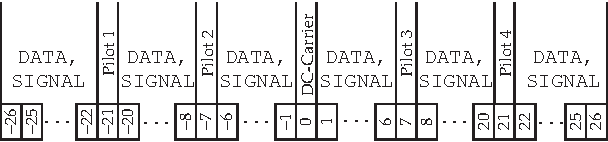
\includegraphics{../kapitel04/figures/OFDM_Sym.pdf}
	\caption{Mapping of the subcarriers}
	\label{fig:OFDM_Sym}
\end{figure}

The standard proposes to transform the subcarriers shown in figure \ref{fig:OFDM_Sym} to the time domain with an \ac{IFFT} of length 64. Therefore, the 53 subcarriers have to be zero padded and shifted in a manner that the DC-carrier is on the first position. After the transformation, the guard interval can be created by prefixing the last 16 values of the output of the \ac{IFFT}. This leads to a length of 80 complex symbols per OFDM symbol and hence a duration of \SI{4}{\micro s}.




\section{Mapping Waveforms to Platforms}
\begin{itemize}
	\item Realization of the PSM for the different development environments and for the different waveforms
\end{itemize}

\section{Model-Based Design on DSP}
\begin{itemize}
	\item Benchmarks of the generated Code with Real Time Workshop and different compilers compared to straight code implementation with C
\end{itemize}

\section{Model-Based Design on FPGA}
\begin{itemize}
	\item Benchmarks of the generated Code with HDL Coder, with System Generator and with a straight hardware description language 
\end{itemize}

\section{High Level Waveform Development on GPP}
\begin{itemize}
	\item Benchmarks of High Level Code connected with Python and CORBA on the one side and generated Code with Real Time Workshop on the other side. Straight C code acts as a reference
\end{itemize}
